\section{Presentation Logic Layer}

%What pages will be present in your project? briefly indicate how your web site will be organized

The website will be divided into the following pages:
\begin{itemize}
    \item Login page: allows the users login to the web application. User must enter their email or username and password for account authentication.
    \item Sign up page: allows the user to register to the web pages. The registration process is divided into 3 different steps/pages where different
    info are requested.
    \begin{itemize}
        \item Personal information page: asks for the user's name, surname, role, brand name, birth date and a recommended profile image.
        \item Address information page: asks for the user's address, city, country and post code.
        \item Account information page: asks to insert the username, email and password for the account.
    \end{itemize}
    \item Homepage: shows the most recent art pieces uploaded by the artists the logged user is following. Also 
    allows user to follow new artists by searching them by username.
    \item Profile settings page: allows user to edit their account info and to access their order history and following 
    lists, which are shown in separate pages.
    \item Artist profile page: is a space managed by an artist where his/her info are shown. Is divided into 3 sections:
    \begin{itemize}
        \item Showcase section: accessed by other users to see a complete list of the artist uploaded art pieces.
        \item Shop section: accessed by other users to potentially buy an art piece being sold by the artist.
        \item Biography section: accessed by other users to get to know more about the artist the profile belongs to.
    \end{itemize}
    \item Art gallery profile page: is similar to the previous described page, but it has only two sections:
    \begin{itemize}
        \item Showcase section: accessed by other users to see the events held in the art gallery.
        \item Biography section: accessed by other users to get to know more about the art gallery the profile belongs 
        to.
    \end{itemize}
    \item Art piece page: displays additional info about an art piece. If it is being sold also allows access to a buy option, which leads to the order page.
    \item Order page: allows the user to buy an art piece. The user will se a summary of the order and will be asked to pay using his PayPal account.
    \item Order history page: shows the user's order history. To simplify the search for a specific order, the user can filter the orders by date or cost. 
\end{itemize}

Each page, except for the login and the signup page, includes a side navigation bar that allows the user to quickly access his homepage, the notification list, the settings page and the profile page.

%%%%%%%%%%%%%%%%%%%%%%%%%%%%%%%%%%%%%%%%%%%%%%%%%%%%%%%
\subsection{Login page (Interface Mokups)}
\begin{figure}[H]
    \centering
    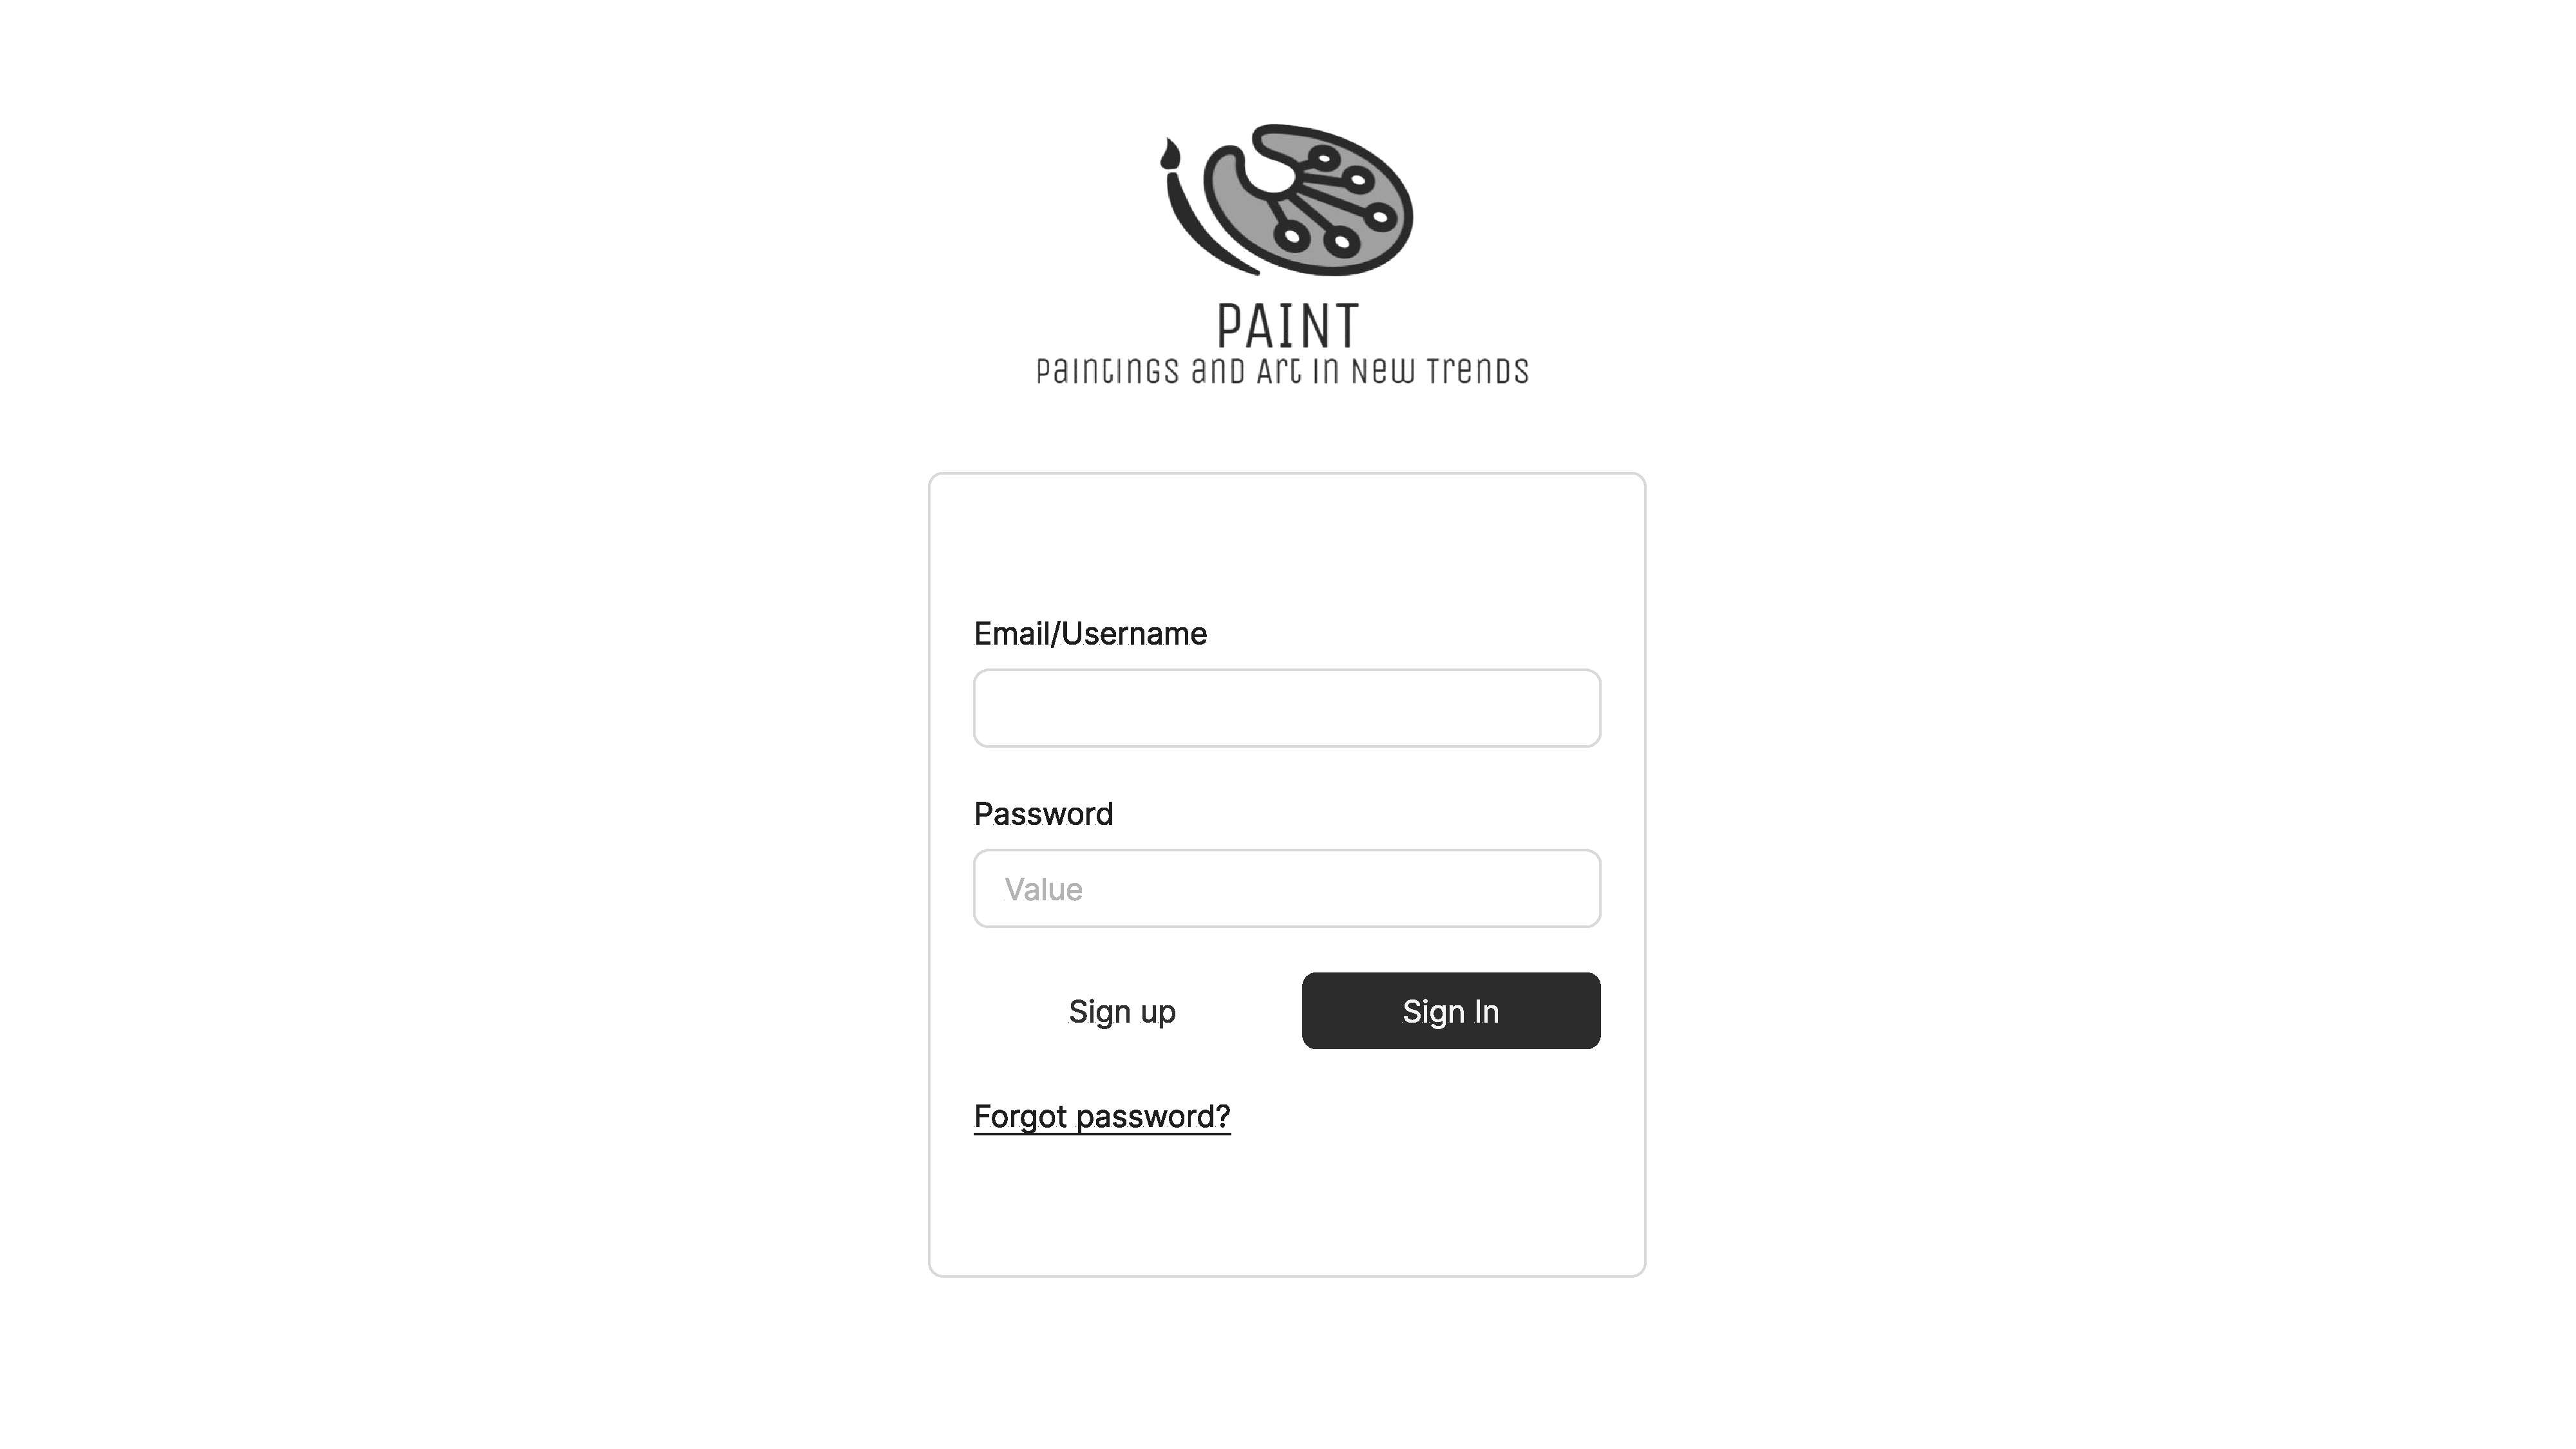
\includegraphics[width=0.5\textwidth]{images/interface_mockups/Landing page - login.pdf}
    \caption{Login page}
\end{figure}

On the login page, users can enter their email and password to authenticate their account and access the web application. If a user forgets their password, they have the option to request a reset link, which will be sent to their registered email. Once successfully logged in, users are redirected to the homepage.

%%%%%%%%%%%%%%%%%%%%%%%%%%%%%%%%%%%%%%%%%%%%%%%%%%%%%%%
\subsection{Signup page (Interface Mokup)}
\begin{figure}[H]
    \centering
\begin{subfigure}[b]{0.49\textwidth}
    \centering
    \includegraphics[width=\textwidth]{images/interface_mockups/Landing page - sign up - personal information.pdf}
    \caption{Personal information page}
\end{subfigure}
\begin{subfigure}[b]{0.49\textwidth}
    \centering
    \includegraphics[width=\textwidth]{images/interface_mockups/Landing page - sign up - address information.pdf}
    \caption{Address information page}
\end{subfigure}
\begin{subfigure}[b]{0.49\textwidth}
    \centering
    \includegraphics[width=\textwidth]{images/interface_mockups/Landing page - sign up - account information.pdf}
    \caption{Account information page}
\end{subfigure}
\end{figure}

The sign-up process is divided into three steps to collect detailed user information. In the first step, users provide their personal information, including name, surname, role, date of birth, and an optional profile image. If the selected role is 'Art gallery' or 'Business user', the user is required to insert the Brand name. 
The second step collects address details such as street address, city, country, and postal code. 
In the final step, users create their account by selecting a username, providing an email, and setting a password that meets security requirements.
By clicking the "Sign up" button, the user's information is validated and stored in the database.
Upon successful registration, users are redirected to the login page to access their new account.


    
%%%%%%%%%%%%%%%%%%%%%%%%%%%%%%%%%%%%%%%%%%%%%%%%%%%%%%%
\subsection{Homepage (Interface Mokup)}
\begin{figure}[H]
    \centering
    \includegraphics[width=0.5\textwidth]{images/interface_mockups/Home - regular users.pdf}
    \caption{Homepage for regular users}
\end{figure}

The homepage displays the most recent art pieces uploaded by artists and art galleries the user follows. 
Users can also search for new artists by their username and follow them. 
A side navigation bar on the left provides quick access to notifications, settings, and the user’s profile, while on the right, users can see popular profiles on the platform and quickly follow them.

%%%%%%%%%%%%%%%%%%%%%%%%%%%%%%%%%%%%%%%%%%%%%%%%%%%%%%%
\subsection{Profile settings page (Interface Mokup)}
\begin{figure}[H]
    \centering
    \includegraphics[width=0.5\textwidth]{images/interface_mockups/Profile settings - main page.pdf}
    \caption{Profile settings main page}
\end{figure}

On the profile settings page, users can update their personal and account information. Additionally, they can navigate to their order history and the list of followed artists, each available on separate pages. The page ensures users maintain control over their preferences and past interactions.

%%%%%%%%%%%%%%%%%%%%%%%%%%%%%%%%%%%%%%%%%%%%%%%%%%%%%%%
\subsection{Artist profile page (Interface Mokup)}
\begin{figure}[H]
    \centering
\begin{subfigure}[b]{0.49\textwidth}
    \centering
    \includegraphics[width=\textwidth]{images/interface_mockups/Artist profile - showcase.pdf}
    \caption{Artpieces showcase page}
\end{subfigure}
\begin{subfigure}[b]{0.49\textwidth}
    \centering
    \includegraphics[width=\textwidth]{images/interface_mockups/Artist profile - shop.pdf}
    \caption{Shop section}
\end{subfigure}
\begin{subfigure}[b]{0.49\textwidth}
    \centering
    \includegraphics[width=\textwidth]{images/interface_mockups/Artist profile - bio.pdf}
    \caption{Artist biography page}
\end{subfigure}
\end{figure}


%%%%%%%%%%%%%%%%%%%%%%%%%%%%%%%%%%%%%%%%%%%%%%%%%%%%%%%
\subsection{Art gallery profile page (Interface Mokup)}
\begin{figure}[H]
    \centering
\begin{subfigure}[b]{0.49\textwidth}
    \centering
    \includegraphics[width=\textwidth]{images/interface_mockups/Art gallery profile - showcase.pdf}
    \caption{Art gallery showcase page}
\end{subfigure}
\begin{subfigure}[b]{0.49\textwidth}
    \centering
    \includegraphics[width=\textwidth]{images/interface_mockups/Art gallery profile - bio.pdf}
    \caption{Art gallery biography page}
\end{subfigure}
\end{figure}


%%%%%%%%%%%%%%%%%%%%%%%%%%%%%%%%%%%%%%%%%%%%%%%%%%%%%%%
\subsection{Art piece page (Interface Mokup)}
\begin{figure}[H]
    \centering
    \includegraphics[width=0.5\textwidth]{images/interface_mockups/Art piece page.pdf}
    \caption{Art piece page}
\end{figure}

The art piece page provides detailed information about a specific artwork, including its title, artist, creation date, dimensions, weight, and description. If the artwork is available for sale, the page displays its price and includes an option to proceed with a purchase, leading the user to the order page.


%%%%%%%%%%%%%%%%%%%%%%%%%%%%%%%%%%%%%%%%%%%%%%%%%%%%%%%
\subsection{Order page (Interface Mokup)}
\begin{figure}[H]
    \centering
    \includegraphics[width=0.5\textwidth]{images/interface_mockups/Order page.pdf}
    \caption{Order page}
\end{figure}

On the order page, users can review their purchase details, including the selected art piece and its cost. They must provide shipping information such as name, surname, email, country, city, postal code, and address. After reviewing the total order amount, users can proceed with the payment using their PayPal account.


%%%%%%%%%%%%%%%%%%%%%%%%%%%%%%%%%%%%%%%%%%%%%%%%%%%%%%%
\subsection{Order history page (Interface Mokup)}
\begin{figure}[H]
    \centering
    \includegraphics[width=0.5\textwidth]{images/interface_mockups/Order History.pdf}
    \caption{Order history page}
\end{figure}

The order history page allows users to view their past purchases. Each order entry includes details such as the order number, purchase date, product name, and cost. To facilitate navigation, users can filter orders by date or cost. The page ensures users can easily track their transactions and retrieve information about previous purchases.